\documentclass[%
pdf,
%nocolorBG,
colorBG,
slideColor,
tcrico,
%slideBW,
%draft,
%frames
%azure
%contemporain
%nuancegris
%troispoints
%lignesbleues
%darkblue
%alienglow
%autumn
%default
%gyom
%blends
]{prosper}
\usepackage{amsmath}
%\usepackage[table]{xcolor}
\usepackage{colortbl}
\usepackage{graphicx}


\begin{document}

\begin{slide}{Knowledge Based Technologies}
\large
\textbf{Lecture 1} 
\newline
\textbf{Introduction}

\bigskip
\small
John Moore \& Thomas Collins



\end{slide}

%%%%%%%%%%%%%%%%%%%%%%%%%%%%%%%%


\begin{slide}{Lecture Overview}
\begin{itemize}
\item Aims \& Objectives
\item Module delivery 
\item Associated resources
\item Assessment
\item Lecture topics 
\item Field overview \& background material
\end{itemize}
\end{slide}

%%%%%%%%%%%%%%%%%%%%%%%%%%%%%%%%


\begin{slide}{Module Delivery}
\begin{itemize}
\item Lectures \& Seminars
	\begin{itemize}
	\item Monday am
	\end{itemize}
\item Relevant material disseminated through Blackboard
\item Self study required
\end{itemize} 
\end{slide}

%%%%%%%%%%%%%%%%%%%%%%%%%%%%%%%%



\begin{slide}{Resources}
\begin{itemize}
\item Material is available week-by-week on Blackboard.
\item Material will be introduced in the lecture/tutorial.
\item Detailed information about the module is found in the MSG on BB.
\item Other material is available in the MSG and via referenced textbooks
\end{itemize}
\end{slide}

%%%%%%%%%%%%%%%%%%%%%%%%%%%%%%%%


\begin{slide}{Assessment}
\begin{itemize}
\item One in module assessment
	\begin{itemize}
	\item Research orientated 
	\end{itemize}
\item Written end of semester exam 
\item More information available in the MSG
\end{itemize}
\end{slide}

%%%%%%%%%%%%%%%%%%%%%%%%%%%%%%%%



\begin{slide}{Lecture Topics}
\tiny
\begin{enumerate}
 \item Introduction/Overview
\item General to specific classification (Introduction to concept learning)
\item Computational Decision making (Overview of Decision tree based learning).
\item Knowledge and Reasoning (An introduction to Neural Networks )
\item Reasoning in light of uncertain knowledge (An introduction to Bayesian learning)
\item Evolutionary learning (An Introduction to Genetic Algorithms)
\item Exploiting contextual knowledge (An Introduction to Instance-Based Learning)
\item Review including comparison/contrast of techniques dealt with to this point.
\item Case based learning (Instance-Based learning overview).
\item Explanation based learning (Analytical learning overview).
\item Knowledge Evaluation (Evaluating hypotheses).
\item Learning from acquired feedback (Reinforcement Learning).
\item Practical applications of techniques.
\item Review
\end{enumerate}
\end{slide}

%%%%%%%%%%%%%%%%%%%%%%%%%%%%%%%%

\begin{slide}{Knowledge}
\begin{itemize}
 \item The sum or range of what has been perceived, discovered, or learned.
\begin{itemize}
 \item Aspects
 \item Structure 
\item Features
\item Context
\end{itemize}
\item \textbf{Question:} Given these aspects list some knowledge sources you are familiar with?
\end{itemize}
\end{slide}
%%%%%%%%%%%%%%%%%%%%%%%%%%%%%%%%


\begin{slide}{Knowledge Representation}
\tiny
\begin{itemize}
 \item  Language (symbolism)
	\begin{itemize}
	\item What format should form the basis of any representation e.g. mathematical, natural language etc?
	\end{itemize}
\item Ontology 
	\begin{itemize}
	\item Representing the concepts within a domain and their inter-relationships.
	\end{itemize}
\item Links and structures
	\begin{itemize}
	\item Structural representation e.g. tabular, tree based etc?
	\end{itemize}
\item Notation
	\begin{itemize}
	\item XML, text, formulae etc 
	\end{itemize}
\item Storage and manipulation
	\begin{itemize}
	\item Semantic nets, frames ect 
	\item The type of storage used has a direct impact on task accomplishment
	\end{itemize}
\end{itemize}
\end{slide}

%%%%%%%%%%%%%%%%%%%%%%%%%%%%%%%%

\begin{slide}{The Goal of Knowledge Manipulation}
\begin{itemize}
 \item  Extract 'useful' information from domain data
	\begin{itemize}
	\item \textbf{Question:} What do you think 'useful' means in this context?
	\end{itemize}
\end{itemize}
\end{slide}

%%%%%%%%%%%%%%%%%%%%%%%%%%%%%%%%


\begin{slide}{Knowledge Based Technologies}
\begin{itemize}
 \item  Technologies that support the extraction and manipulation of data with the aim of reaching a desired goal.
	\begin{itemize}
	\item Algorithms
		\begin{itemize}
			\item AI
			\item Ability to 'learn'
		\end{itemize}
	\item Encapsulating software 
		\begin{itemize}
		\item Commoditised software 
			\begin{itemize}
			\item e.g. Gaming, Customer profiling etc
			\end{itemize}
		\end{itemize}
	\end{itemize}
\end{itemize}
\end{slide}

%%%%%%%%%%%%%%%%%%%%%%%%%%%%%%%%

\begin{slide}{Artificial Intelligence}
\begin{itemize}
 \item  Somewhat controversial issue historically.
	\begin{itemize}
	\item \textbf{Question:} What is your definition of AI? 
	\end{itemize}
 \item There can be considered four views of what AI is:
	\begin{center}
	\begin{tabular}{c||c}
	\rowcolor[HTML]{aabbcc}\textbf{Thinking in a } & \textbf{Thinking in a} \\
	\rowcolor[HTML]{aabbcc}\textbf{human manner} & \textbf{rational manner}\\ \hline \hline
	\rowcolor[HTML]{aabbcc}\textbf{Acting in a } & \textbf{Acting in a} \\
	\rowcolor[HTML]{aabbcc}\textbf{human manner} & \textbf{rational manner}\\ 
	\end{tabular}
	\end{center}
 \item In this context we focus on the emergence of rational actions.
\end{itemize}
\end{slide}

%%%%%%%%%%%%%%%%%%%%%%%%%%%%%%%%


\begin{slide}{Acting humanly: Turing Test}
\begin{itemize}
 \item  Turing (1950) ''Computing machinery and intelligence'':
	\begin{itemize}
	\item Can machines think? $\xrightarrow{}$ Can machines behave intelligently?
	\item Operational test for intelligent behaviour: \textit{The Imitation Game}
	\begin{figure}
	\centering
	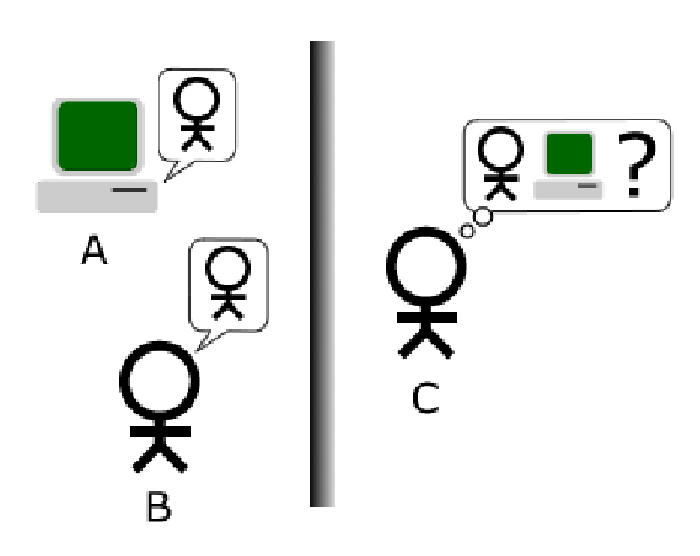
\includegraphics[scale=0.3]{Turing_Test_version_4.eps}
	\end{figure}
	\end{itemize}
\item Suggested major components of AI: knowledge, reasoning, language understanding, learning
\end{itemize}
\end{slide}

%%%%%%%%%%%%%%%%%%%%%%%%%%%%%%%%

\begin{slide}{Thinking humanly: Cognitive modelling}
\footnotesize 
\begin{itemize}
 \item 1960s ''Cognitive revolution'': information-processing psychology 
 \item Requires scientific theories of internal activities of the brain.
	\begin{itemize}
 	\item  How to validate? Requires: 
		\begin{enumerate}
 		\item Predicting and testing behaviour of human subjects (top-down) \textbf{or}
   		\item Direct identification from neurological data (bottom-up)
		\end{enumerate}
	\end{itemize}
 \item  Both approaches (Cognitive Science and Cognitive Neuroscience) are now distinct from AI. The following characteristic is shared however:
	\begin{itemize}
		\item \textit{The available theories do not explain anything resembling human-level general intelligence!}
	\end{itemize}
\end{itemize}
\end{slide}


%%%%%%%%%%%%%%%%%%%%%%%%%%%%%%%%
\begin{slide}{Thinking rationally: ''Laws of thought''}
\tiny
\begin{itemize}
 \item Prescriptive rather than descriptive.
 \item Aristotle: ''What are correct arguments/thought processes?''
\item Several Greek schools developed various forms of logic: 
	\begin{itemize}
	\item Notation and rules of derivation for thoughts;
	\item May or may not have proceeded to the idea of mechanization
	\end{itemize}
\item Direct line through mathematics and philosophy to modern AI
\item Issues:
	\begin{enumerate}
	\item Not all intelligent behaviour is mediated by logical deliberation
	\item What is the purpose of thinking? What thoughts should I have?
	\end{enumerate}
\end{itemize}
\end{slide}

%%%%%%%%%%%%%%%%%%%%%%%%%%%%%%%%
\begin{slide}{Acting Rationally}
\begin{itemize}
 \item Acting
	\begin{itemize}
	\item Catch-all term meaning the observed emergent behaviour 
	\end{itemize}
\item Rational
	\begin{itemize}
	\item Maximise benefit at each stage/during each operational condition.
	\end{itemize}
\item Doesn't necessarily involve thinking!
	\begin{itemize}
	\item e.g. blinking reflex 
	\end{itemize}
\item However ‘thinking’ should be in the service of rational action 
\end{itemize}
\end{slide}


%%%%%%%%%%%%%%%%%%%%%%%%%%%%%%%%
\begin{slide}{Rational Agents}
\begin{itemize}
 \item An agent is an entity that perceives and acts.
	\begin{itemize}
	\item e.g. a web spider, a dedicated analysis algorithm etc
	\end{itemize}
\item For any given class of environments and tasks, we seek the agent (or class of agents) with the best performance.
\item However domain and computational limitations make perfect rationality unachievable.
\item Agents need to be provided with the capabilities to deal with such limitations.
	\begin{itemize}
	\item Machine Learning
	\end{itemize}
\end{itemize}
\end{slide}



%%%%%%%%%%%%%%%%%%%%%%%%%%%%%%%%
\begin{slide}{Machine Learning}
\begin{itemize}
 \item Discipline that is concerned with the design and development of algorithms that allow computers to learn based on data.
	\begin{itemize}
	\item Automatically learn to recognize complex patterns and make intelligent decisions based on data.
	\end{itemize}
\item \textbf{Question:} What does intelligent mean in this context?
\end{itemize}
\end{slide}


%%%%%%%%%%%%%%%%%%%%%%%%%%%%%%%%
\begin{slide}{Domain Categories}
\begin{itemize}
 \item Supervised learning
	\begin{itemize}
	\item Map from a known set of inputs to a desired output.
		\begin{itemize}
		\item e.g. Simplistic currency trend prediction.
		\end{itemize}
	\end{itemize}
 \item Unsupervised learning
	\begin{itemize}
	\item Learn classifications from unlabelled input.
		\begin{itemize}
		\item e.g. Amazon book recommendation system.
		\end{itemize}
	\end{itemize}
 \item Semi-supervised learning
	\begin{itemize}
	\item Given some domain assumptions learn classifications an unlabelled data set.
		\begin{itemize}
		\item e.g. Bioinformatics applications.
		\end{itemize}
	\end{itemize}
\end{itemize}
\end{slide}

%%%%%%%%%%%%%%%%%%%%%%%%%%%%%%%%
\begin{slide}{Domain Categories ctd}
\begin{itemize}
 \item Reinforcement learning.
	\begin{itemize}
	\item Learn based on observations of  the domain.
		\begin{itemize}
		\item e.g. Robotics.
		\end{itemize}
	\end{itemize}
\item Transduction.
	\begin{itemize}
	\item Attempt to predict new outputs based on all available information.
	\end{itemize}
\item Learning to learn
\end{itemize}
\end{slide}


%%%%%%%%%%%%%%%%%%%%%%%%%%%%%%%%
\begin{slide}{Application Areas}
\footnotesize
\begin{itemize}
 \item Industrial applications of the techniques highlighted previously.
\item These techniques continue to evolve and find wider acceptance and adoption.
	\begin{itemize}
	\item Why?
	\end{itemize}
\item Sample application areas
	\begin{itemize}
	\item Customer Relationship management.
	\item Electrical power engineering
	\item Trend analysis 
		\begin{itemize}
		\item e.g. Swine flu 
		\end{itemize}
\item Surveillance
	\end{itemize}
\end{itemize}
\end{slide}


%%%%%%%%%%%%%%%%%%%%%%%%%%%%%%%%
\begin{slide}{Review}
\tiny
\begin{itemize}
 \item The concept of knowledge.
\item Knowledge representation.
	\begin{itemize}
	\item Goals 
	\item Challenges
	\end{itemize}
\item Computationally accommodating knowledge and it's elicitation 
	\begin{itemize}
	\item AI
	\item Machine  Learning
	\end{itemize}
\item Available knowledge as domain categorisation facilitators 
	\begin{itemize}
	\item The knowledge available influences the approach chosen to manipulate the domain data 
	\end{itemize}
\item Application areas 
\item Next week: Inductive learning \dots

\end{itemize}
\end{slide}


\end{document}
